\chapter{{\LaTeX} test}

This \LaTeX template is configured to produce a PDF.
Your figures should be PDF files like Figure~\ref{fig:pdf}.
If you do not have a PDF version of your figure, \emph{latexmk} and \emph{emph} can convert the image to PDF for you as shown in Figure~\ref{fig:svg}.

\begin{figure}
  \centering
  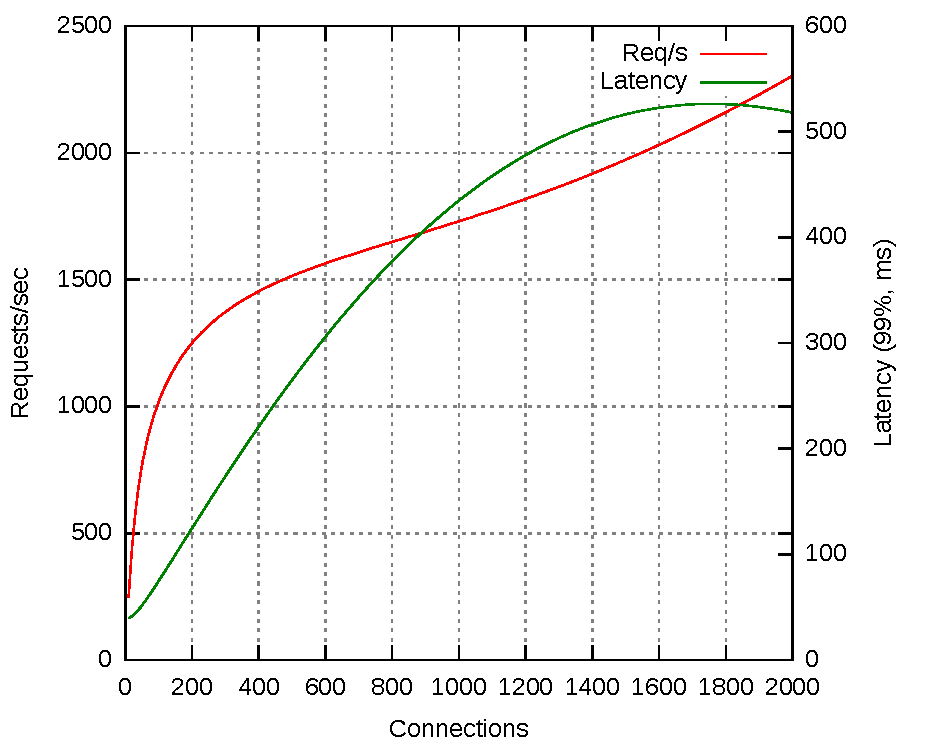
\includegraphics{figures/just-a-plot}
  \caption[Figures must be PDF]{All figures must be PDFs.}
  \label{fig:pdf}
\end{figure}

\begin{figure}
  \centering
  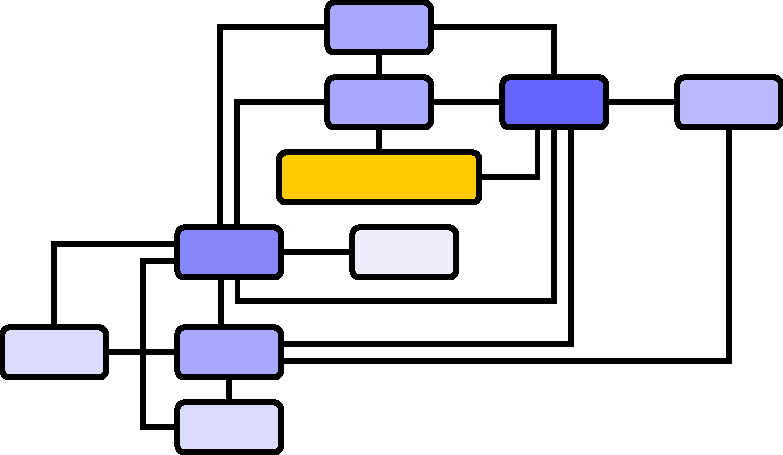
\includegraphics{figures/just-a-graph}
  \caption[SVG converted to PDF]{the \texttt{Makefile} and \texttt{latexmkrc} files include a rule to convert SVG images to PDF images.
	\emph{latexmk} will convert EPS files for you too.}
  \label{fig:svg}
\end{figure}

\begin{equation}
    \label{eq:maxwell}
    \begin{aligned}
    \frac{\partial\mathcal{D}}{\partial t} & = \nabla\times\mathcal{H},   & \text{(Loi de Faraday)}\\
    \frac{\partial\mathcal{B}}{\partial t} & = -\nabla\times\mathcal{E},  & \text{(Loi d'Ampère)}\\
    \nabla\cdot\mathcal{B}                 & = 0,                         & \text{(Loi de Gauss)}\\
    \nabla\cdot\mathcal{D}                 & = 0.                         & \text{(Loi de Colomb)}
    \end{aligned}
\end{equation}

\[
    \oint_C {E \cdot d\ell = - \frac{d}{{dt}}} \int_S {B_n dA}
\]

L45 = \the\xlvchars\par
L65 = \the\lxvchars

\clearpage
\layout
